\documentclass{article}[18pt]
\ProvidesPackage{format}
%Page setup
\usepackage[utf8]{inputenc}
\usepackage[margin=0.7in]{geometry}
\usepackage{parselines} 
\usepackage[english]{babel}
\usepackage{fancyhdr}
\usepackage{titlesec}
\hyphenpenalty=10000

\pagestyle{fancy}
\fancyhf{}
\rhead{Sam Robbins}
\rfoot{Page \thepage}

%Characters
\usepackage{amsmath}
\usepackage{amssymb}
\usepackage{gensymb}
\newcommand{\R}{\mathbb{R}}

%Diagrams
\usepackage{pgfplots}
\usepackage{graphicx}
\usepackage{tabularx}
\usepackage{relsize}
\pgfplotsset{width=10cm,compat=1.9}
\usepackage{float}

%Length Setting
\titlespacing\section{0pt}{14pt plus 4pt minus 2pt}{0pt plus 2pt minus 2pt}
\newlength\tindent
\setlength{\tindent}{\parindent}
\setlength{\parindent}{0pt}
\renewcommand{\indent}{\hspace*{\tindent}}

%Programming Font
\usepackage{courier}
\usepackage{listings}
\usepackage{pxfonts}

%Lists
\usepackage{enumerate}
\usepackage{enumitem}

% Networks Macro
\usepackage{tikz}


% Commands for files converted using pandoc
\providecommand{\tightlist}{%
	\setlength{\itemsep}{0pt}\setlength{\parskip}{0pt}}
\usepackage{hyperref}

% Get nice commands for floor and ceil
\usepackage{mathtools}
\DeclarePairedDelimiter{\ceil}{\lceil}{\rceil}
\DeclarePairedDelimiter{\floor}{\lfloor}{\rfloor}

% Allow itemize to go up to 20 levels deep (just change the number if you need more you madman)
\usepackage{enumitem}
\setlistdepth{20}
\renewlist{itemize}{itemize}{20}

% initially, use dots for all levels
\setlist[itemize]{label=$\cdot$}

% customize the first 3 levels
\setlist[itemize,1]{label=\textbullet}
\setlist[itemize,2]{label=--}
\setlist[itemize,3]{label=*}

% Definition and Important Stuff
% Important stuff
\usepackage[framemethod=TikZ]{mdframed}

\newcounter{theo}[section]\setcounter{theo}{0}
\renewcommand{\thetheo}{\arabic{section}.\arabic{theo}}
\newenvironment{important}[1][]{%
	\refstepcounter{theo}%
	\ifstrempty{#1}%
	{\mdfsetup{%
			frametitle={%
				\tikz[baseline=(current bounding box.east),outer sep=0pt]
				\node[anchor=east,rectangle,fill=red!50]
				{\strut Important};}}
	}%
	{\mdfsetup{%
			frametitle={%
				\tikz[baseline=(current bounding box.east),outer sep=0pt]
				\node[anchor=east,rectangle,fill=red!50]
				{\strut Important:~#1};}}%
	}%
	\mdfsetup{innertopmargin=10pt,linecolor=red!50,%
		linewidth=2pt,topline=true,%
		frametitleaboveskip=\dimexpr-\ht\strutbox\relax
	}
	\begin{mdframed}[]\relax%
		\centering
		}{\end{mdframed}}



\newcounter{lem}[section]\setcounter{lem}{0}
\renewcommand{\thelem}{\arabic{section}.\arabic{lem}}
\newenvironment{defin}[1][]{%
	\refstepcounter{lem}%
	\ifstrempty{#1}%
	{\mdfsetup{%
			frametitle={%
				\tikz[baseline=(current bounding box.east),outer sep=0pt]
				\node[anchor=east,rectangle,fill=blue!20]
				{\strut Definition};}}
	}%
	{\mdfsetup{%
			frametitle={%
				\tikz[baseline=(current bounding box.east),outer sep=0pt]
				\node[anchor=east,rectangle,fill=blue!20]
				{\strut Definition:~#1};}}%
	}%
	\mdfsetup{innertopmargin=10pt,linecolor=blue!20,%
		linewidth=2pt,topline=true,%
		frametitleaboveskip=\dimexpr-\ht\strutbox\relax
	}
	\begin{mdframed}[]\relax%
		\centering
		}{\end{mdframed}}
\lhead{MCS - Logic and Discrete Structures}


\begin{document}
\begin{center}
\underline{\huge More on Natural Deduction for Propositional Logic}
\end{center}
\section{More rules}
\begin{itemize}
	\item Rules for introducing disjunction\\
	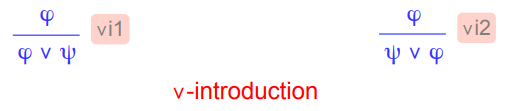
\includegraphics[scale=0.7]{v-introduction.png}
	\item Rules for eliminating disjunction\\
	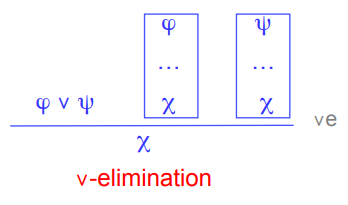
\includegraphics[scale=0.7]{v-elimination.png}\
	\item In order to apply the rule $\lor$e, we use boxes as previously
	\begin{itemize}
		\item But now there is a box starting with each disjunct $\varphi$ and $\psi$
		\item Each box needs to end with the same intended formula, $\chi$
	\end{itemize}
\end{itemize}
\section{A proof using $\lor$ elimination}
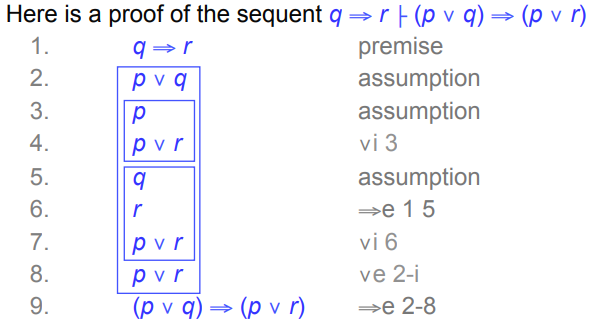
\includegraphics[scale=0.7]{v_proof1.png}\\
\begin{itemize}
	\item Assume that p is true, so the RHS is true
	\item $p\lor r$ is true
	\item Open box assuming q is true
	\item Eliminate the implies symbol from the LHS
	\item Shown that no matter if p or q is true, the statement $p\lor r$ will be true
	\item It has been shown that if $p\lor q$ is true, that $p\lor r$ is true, so $(p\lor q)\Rightarrow (p\lor r)$ will always be true
\end{itemize}
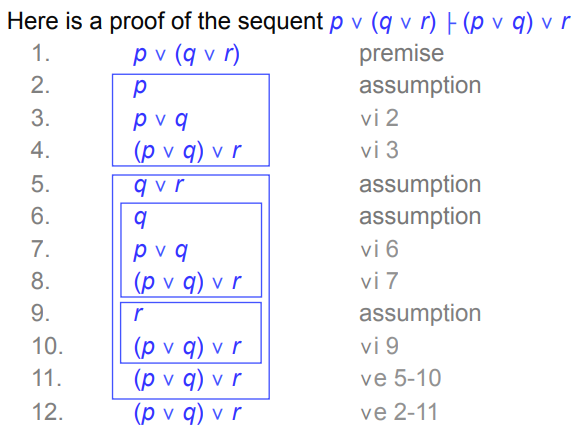
\includegraphics[scale=0.7]{v_proof2.png}
\begin{itemize}
	\item Basically trying to build the RHS from the LHS
\end{itemize}
\section{More rules}
\begin{itemize}
	\item Rules for negation\\
	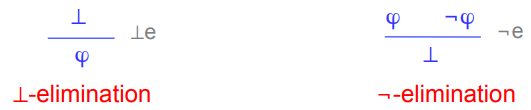
\includegraphics[scale=0.7]{negation_rules.png}
	\item The symbol $\bot$, known as bottom, represents a contradiction, in natural deduction if one has a contradiction then one can infer \textbf{any} formula
	\item Rules for introducing negation\\
	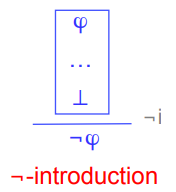
\includegraphics[scale=0.7]{introduce_negation.png}
\end{itemize}
\section{A proof using rules for negation}
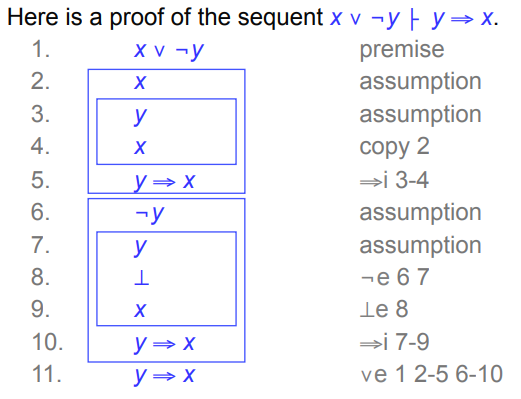
\includegraphics[scale=0.7]{negation_proof1.png}
\begin{itemize}
	\item $p\land\lnot p\Rightarrow \varphi$ holds as $p\land\lnot p$ will always be false, and if the LHS of an implication is false, then the whole statement will be true 
	\item Lines $2\rightarrow 5$ say $x\Rightarrow(y\Rightarrow x)$
\end{itemize}
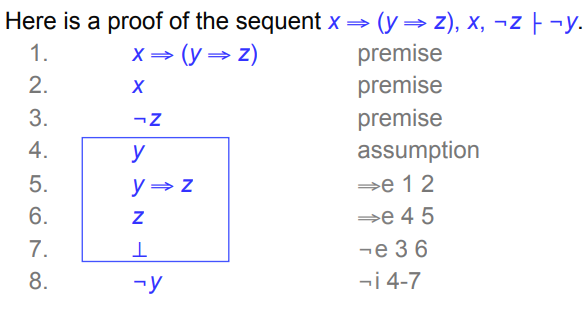
\includegraphics[scale=0.7]{negation_proof2.png}
\section{A derived rule}
\begin{itemize}
	\item We can derive other rules in natural deduction 
	\item Consider modus tollens $\varphi\Rightarrow\psi, \lnot\psi\vdash\lnot\varphi$ \\
	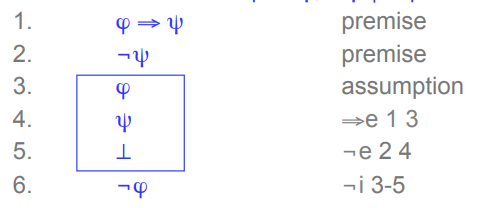
\includegraphics[scale=0.7]{modus_tollens.png}
	\item Note that we can use derived rules just as if they were rules of natural deduction
	\begin{itemize}
		\item e.g., in a proof with
		\begin{itemize}
			\item a line reading $\varphi\Rightarrow\psi$
			\item and another line reading $\lnot\psi$
		\end{itemize}
		\item we could immediately infer $\lnot\psi$ and write modus tollens as an explaining remark
	\end{itemize}
\end{itemize}

\section{More derived rules}
\begin{itemize}
	\item Proof by contradiction is the principle "if from $\lnot\varphi$ I can prove $\bot$ then I can deduce $\varphi$
	\item Here is a proof that this principle can be applied in natural deduction\\
	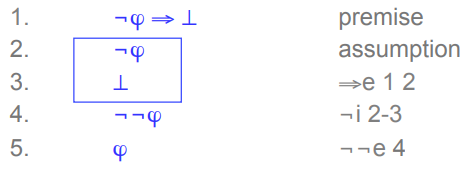
\includegraphics[scale=0.7]{ProofByContradiction.png}
	\item We denote reductio ad absurdum by RAA
\end{itemize}
\section{More derived rules}
\begin{itemize}
	\item The law of excluded middle states that either $\varphi$ is true or $\lnot\varphi$ is true
	\item Here is a proof of it\\
	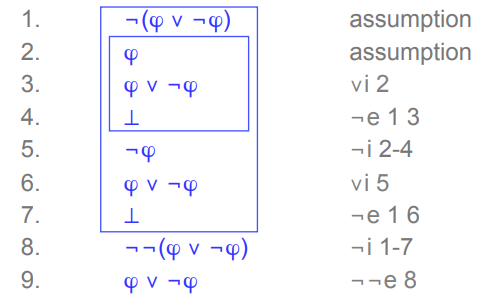
\includegraphics[scale=0.7]{MiddleStates.png}
	\item We denote the law of excluded middle by LEM
\end{itemize}
\section{Some facts about Natural Deduction}
\begin{itemize}
	\item Natural deduction is sound and complete
	\item Let $\varphi_1,\varphi_2,...,\varphi_m$ and $\psi$ be formulae
	\item Soundness
	\begin{itemize}
		\item If the sequent $\varphi_1,\varphi_2,...\varphi_m\vdash\psi$ is provable then the formula $\varphi_1\land\varphi_2\land...\land\varphi_m\Rightarrow\psi$ is a tautology
	\end{itemize}
	\item Completeness
	\begin{itemize}
		\item If $\varphi_1\land\varphi_2\land...\land\varphi_m\Rightarrow\psi$ is a tautology then the sequent $\varphi_1,\varphi_2,...\varphi_m\vdash\psi$ is provable
	\end{itemize} 
	\item A \textbf{theorem} is a formula $\psi$ for which the sequent $\vdash\psi$ is provable, thus, the soundness and completeness of natural deduction tells us that every theorem is a tautology and every tautology is a theorem
\end{itemize}
\section{Proving Theorems}
\begin{itemize}
	\item Here is a proof that the sequent $(p\Rightarrow(\lnot p\lor q))\lor (p\Rightarrow\lnot q)$ is a theorem\\
	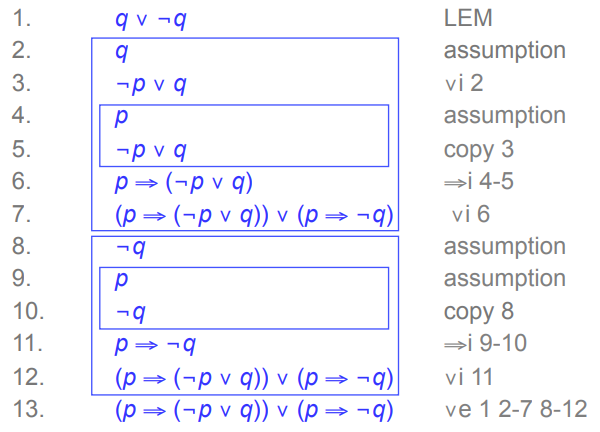
\includegraphics[scale=0.7]{ProvingTheorems}
	
	
\end{itemize}
\end{document}